%; whizzy chapter 
% -initex iniptex -latex platex -format platex -bibtex jbibtex -fmt fmt
% 以上 whizzytex を使用する場合の設定。


%     Tokyo Debian Meeting resources
%     Copyright (C) 2006 Junichi Uekawa

%     This program is free software; you can redistribute it and/or modify
%     it under the terms of the GNU General Public License as published by
%     the Free Software Foundation; either version 2 of the License, or
%     (at your option) any later version.

%     This program is distributed in the hope that it will be useful,
%     but WITHOUT ANY WARRANTY; without even the implied warranty of
%     MERCHANTABILITY or FITNESS FOR A PARTICULAR PURPOSE.  See the
%     GNU General Public License for more details.

%     You should have received a copy of the GNU General Public License
%     along with this program; if not, write to the Free Software
%     Foundation, Inc., 51 Franklin St, Fifth Floor, Boston, MA  02110-1301 USA

%   Pdf作成手順
% dvipdfmx debianmeetingresume200604.dvi
%  preview (shell-command (concat "xpdf " (replace-regexp-in-string "tex$" "pdf"(buffer-file-name)) "&"))
% 画像ファイルを処理するためにはebbを利用してboundingboxを作成。
%(shell-command "cd image200604; ebb *.png")

%%ここからヘッダ開始。

\documentclass[mingoth,a4paper]{jsarticle}
\usepackage[dvipdfmx]{graphicx}
\usepackage{fancybox}
\usepackage{longtable}
\usepackage{ascmac}	% 囲み (screen,itembox)
\usepackage{fancyvrb}   % 囲み Verbatim のために必要
\usepackage[dvipdfmx]{hyperref}
\usepackage{url}

%http://www.naney.org/diki/dk/hyperref.html
%日本語EUC系環境の時
\AtBeginDvi{\special{pdf:tounicode EUC-UCS2}}
%シフトJIS系環境の時
%\AtBeginDvi{\special{pdf:tounicode 90ms-RKSJ-UCS2}}

%% spacing の設定をする。外枠を減らす。
\setlength\headheight{0mm}
\setlength\topmargin{-20mm}
\setlength\headsep{0mm}
\setlength\topskip{3mm}
\setlength\maxdepth{4pt}
\setlength\columnsep{6mm}
\setlength\textheight{252mm}
\setlength\topmargin{-5mm}
\setlength\textwidth{170mm}
\setlength\oddsidemargin{-5mm}
\setlength\evensidemargin{-5mm}

% commandline環境を定義。画面入出力についてはcommandline環境
% で表記する
\newenvironment{commandline}%
{\VerbatimEnvironment
  \begin{Sbox}\begin{minipage}{15cm}\begin{fontsize}{7.3}{7.3} \begin{BVerbatim}}%
{\end{BVerbatim}\end{fontsize}\end{minipage}\end{Sbox}
  \setlength{\fboxsep}{8pt}\fbox{\TheSbox}}


%%% start of santaku
\makeatletter
\newwrite\tf@jqz
\immediate\openout\tf@jqz\jobname.jqz\relax
\makeatother
\newcounter{santakucounter}
\newcommand{\santaku}[5]{%
\addtocounter{santakucounter}{1}

\addtocontents{jqz}{\arabic{santakucounter}. #5\\}
\nopagebreak 問題\arabic{santakucounter}. 
#1\\
\nopagebreak□ A #2\\
\nopagebreak□ B #3\\
\nopagebreak□ C #4
\pagebreak[1]
\hspace{1cm}
\\

}
%%% end of santaku

\newcommand{\emptyspace}{(\underline{\hspace{1cm}})}

\newcommand{\subsubsubsection}[1]{%
\vspace{1zw}{\bf #1}\\}

% sectionをセンタリングする
\makeatletter
  \renewcommand{\section}{\@startsection{section}{1}{\z@}%
    {\Cvs \@plus.5\Cdp \@minus.2\Cdp}% 前アキ
    {.5\Cvs \@plus.3\Cdp}% 後アキ
    {\normalfont\Large\headfont\raggedright\centering}} % style
\makeatother

% section の代わりの環境
\newcommand{\dancersection}[2]{%
\newpage
東京エリアDebian勉強会 2006
\hrule
\vspace{0.5mm}
\hrule
\hfill{}
\includegraphics[width=3cm]{image200502/openlogo-nd.eps}\\
\vspace{-4cm}
\begin{center}
  \section{#1}
\end{center}
\hfill{}#2\hspace{3cm}\space\\
\hrule
\hrule
\vspace{1cm}
}


% BTSの番号を見るためのコマンド
\newcommand{\debianbug}[1]{#1\footnote{\url{http://bugs.debian.org/#1}}}

% for dancerj
\newcommand{\fgref}[1]{図\ref{#1}}
\newcommand{\tbref}[1]{表\ref{#1}}


\begin{document}

\begin{titlepage}

% 毎月変更する部分, 本文の末尾も修正することをわすれずに
\title{
 第15回 東京エリア Debian 勉強会\\事前資料}
\date{2006年4月15日}
\author{Debian勉強会会場係 上川 純一\thanks{Debian Project Official Developer}} 
\maketitle
\thispagestyle{empty}
\end{titlepage}

\newpage
\tableofcontents

\dancersection{Introduction To Debian 勉強会}{上川 純一}

今月のDebian勉強会へようこそ。
これからDebianのあやしい世界に入るという方も、すでにどっぷりとつかってい
るという方も、月に一回Debianについて語りませんか?

目的として下記の二つを考えています。

\begin{itemize}
 \item メールではよみとれない、もしくはよみとってられないような情報を情
       報共有する場をつくる
 \item まとまっていないDebianを利用する際の情報をまとめて、ある程度の塊と
       して出してみる
\end{itemize}

また、東京にはLinuxの勉強会はたくさんありますので、Debianに限定した勉強
会にします。Linuxの基本的な利用方法などが知りたい方は、他でがんばってくださ
い。
Debianの勉強会ということで究極的には参加者全員がDebian Packageを
がりがりと作りながらスーパーハッカーになれるような姿を妄想しています。

Debianをこれからどうするという能動的な展開への土台としての空間を提供し、
情報の共有をしたい、というのが目的です。
次回は違うこと言ってるかもしれませんが、御容赦を。

\subsection{講師紹介}

\begin{itemize}
 \item{上川 純一} 宴会の幹事です。
\end{itemize}

\subsection{事前課題紹介}

今回の事前課題は
「Debianで文書はこうやってつくっています」
というタイトルで200-800文字程度の文章を書いてください。
というものでした。
その課題に対して下記の内容を提出いただきました。

\subsubsection{小室 文さん}
基本的に議事録とかは後々メールに貼付けたり添付したりするので、bluebirdでテキ
スト作成して、他のユーザーを巻き込むような案件での文章はOpen officeを使って
相手がmicrosoft officeを使って開けるように気をつけています。相手がpowerpoint
で開くとかならずレイアウトが崩れている!と嫌みめいたメールが来ますがそこはあ
んまり気にしないようにしてます。後はよくする事がthunderbirdでメール新規作成
をしてドラフトで保存してます。検索が簡単なのとメールでのやり取りが多い&新し
くbluebirdを立ち上げなくていいので、結構便利だと思っています。

\subsubsection{澤田さん}

dpkgとどう接しているかと言われると、

\begin{itemize}
 \item  パッケージを入れた後にどんなファイルが含まれてるか見るために-L
 \item  パッケージを入れてるかを確認するために-l
 \item  ファイルがどのパッケージのものかを確認するために-S
\end{itemize}

ですね。\texttt{-L}でファイル一覧表示→気になったファイルをlvってのをよくやるの
で、それを統合したアプリなんてあるとうれしいのかもしれない。


\subsubsection{三島さん}
Debian 上で書く文書は、プログラムとそれに付随する文書か、あるいは
日記のようなものが多いです。

プログラムの場合、シェルスクリプト等の短いものならば vi (jvim)
を使いますが、長くなるようなら emacs を使います。インデント等は
emacs に頼りきりです。どちらの場合もテキスト端末用のものしか使い
ません。

一方、日記や、思いつきのメモを書くためには hiki と Web ブラウザを
使っています。どこからでも更新・参照でき、最低限の文書構造を表現
できるので Wiki を使っています。難点は、hiki の編集モードが
W-ZERO3 + Opera 環境からだととても使いづらいところです。

\subsubsection{矢吹さん}

Debianの上で生活をしているので、Debianで文書を作成するのは、特別に意識
することなく作成しています。基本的には日本語で文書を作成し、英語で文書
を作成することもあります。
日本語の文書を作成する上で、重要なファクターとして「日本語入力」があり
ます。現在ケースバイケースで複数の日本語入力をおこなっています。現在
Xの上では、SCIMをつかっており、Emacsの上ではyc-elを使っています。
入力方法は、ローマ字ならびにNicola入力で入力することが多いです。
文書は、mailが一番おおく、つぎはtDiaryへのpublishingです。その次は
発表資料作成に、OpenOffice.orgのImpressでプレゼン資料を作ります。
長文の論文などは、\pLaTeX を使います。最終出力形態は、プラットホーム
を意識する場合が少ないpdfにすることが多いです。
英語の文書を作成するときには、辞書とスペルチェッカーが重要です。
ebviewやlookup.el、ならびにflyspell-modeはよく使います。

\subsubsection{吉田@板橋さん}

Debianで文書を作らなければならないときは、
通常、下記いずれかの方法を使用しています。

前提
Cygwinのsshをcocotを使用して起動し、Sarge環境に接続。

\begin{itemize}
 \item 英語の場合 \\
	Windowsでコピーして、viで作成したファイルにi押して貼り付け。
	または\verb!cat >!

 \item 日本語の場合 \\
       jvim-canna-nox(xに依存しない自作野良パッケージ)を使用して
       cannaで入力

 \item 面倒な場合 \\
	scp
\end{itemize}

\subsubsection{中島さん}

文書は、ほとんどWEBブラウザを使って作っていて、テキストの表示も紙に出力しない
でブラウザだけで表示している。ブログを読んでコメントを書いたり全てブラウザを使
う。ワープロや表計算ソフトみたいなのも使わない。簡単な文章やメモ書き程度だった
ら紙で書いている。文字数で言うと400字以内だったら紙を使う。あと漢字変換をや
ってしまうと漢字を忘れるので紙を使うようにしている。それとマインドマップを上手
になりたいので意識的に絵を書くようにしている。紙と色ペンを使って紙で書いてそれ
をブラウザに転記するのがいまのところ一番よい。

\subsubsection{岩松 信洋}
いままで Linux でドキュメントを書くことはありませんでした。プレゼンテーションの
ときは ooimpress でした。しかし、Debian 勉強会に参加して、自分でも発表を行うよう
になってから、\TeX{} に目覚め、今では会社のドキュメントも \TeX{} で書く
ようになってしまいました。これからは Word なんかを使わず、茨の道を進んでいこうと思います。

\subsubsection{やまねさん}
Debianで文章編集…どのような環境、といっても

\begin{itemize}
 \item IME        - uim+anthy
 \item mail        - Sylpheed / firefox(gmail)
 \item irc        - loqui
 \item editor     - gedit / vim
 \item presentation    - OpenOffice.org(Impress)
\end{itemize}

と面白みの無い答えになります。
Emacs など使い方が身につけばつかってみたいのですが、なかなかきっかけがありません。(riece を起動するだけにしか使わない)

\subsubsection{小林さん}

Debianでは主にEmacs 21で文書を書いています。
フォーマットは、個人的なメモなど、
印刷物などにする必要がないものに関してはすべてRDです。

学生なので\TeX{}もそれなりに使ってきました。
レジュメなど最終的に印刷する必要があるものはすべて\TeX{}です。
もちろん修論も同様で、
スタイルファイルにはokumura-clsfilesパッケージのjsbook.clsを使い、
出力はdvipdfmxでpdfに変換しました。
EmacsのメジャーモードにはYa\TeX{}を使っています。

個人的なものについては、印刷物は\TeX{}、それ以外はRDですが、
翻訳作業をしている関係でそれ以外のフォーマットも扱います。
しかし最近では、ウェブページはもちろん、
様々なソフトウェアのドキュメントもみなXML/SGMLやその仲間 (HTML, XHTML, DocBook/XML, wml, ...) で書かれているので、
特筆することはありません。
せいぜい、DocBook/XMLで書かれたAptitudeのドキュメントをdocbook-xslパッケージのXSLTスタイルシートで変換しようとして文字コードやその他のバグにちょっと苦しんだくらいです。
docbook-xslの新しいバージョンのパッケージはいつ入るのかが気になる昨今です (というかsargeリリース直前に入ったのもNMUだし、ほとんどメンテナンスされていないような気がします)。


\subsubsection{北原さん}
  率直に正直に言いますと「Debianで文書はつくって
いません」。 文章を作るときには、手馴れた某OSの某
エディタを使用し、必要があれば、転送・文字コード変
換等を行います。 装飾が必要なときは、作成したテキ
ストをワードプロセッサに読み込ませます。
  これでは、デビアン勉強会の宿題回答にはならない
ので、あえてデビアン環境で文章を作るならという事で
回答すると、短いメモや覚書程度なら vi 、少々サイズ
が大きい文章なら OpenOffice.org でしょうか。 \TeX
とかは使用できません。
(何とか200文字を越えました。)



\subsubsection{上川}

\begin{itemize}
 \item 簡単な文章 \\
       簡単な文書は、最近はoutline-modeで書いています。
       以前はtexであらゆるメモを書いていましたが、最近はフォーマットをあ
       まり考えなくなりました。
 \item 英語での複雑な文章 \\
       英語の文書はDocBookを使う事が多いです。
       emacsでwysidocbookxmlを利用して、リアルタイムプリビューしながらド
       キュメントを書いています。
 \item 日本語での複雑な文章 \\
       whizzytexを利用してリアルタイムプリビューをしながら、texで書いて
       います。
\end{itemize}

%%% trivia quiz
\dancersection{Debian Weekly News trivia quiz}{上川 純一}

ところで、Debian Weekly News (DWN)は読んでいますか?
Debian 界隈でおきていることについて書いているDebian Weekly News.
毎回読んでいるといろいろと分かって来ますが、一人で読んでいても、解説が少
ないので、
意味がわからないところもあるかも知れません。みんなでDWNを読んでみましょう。

漫然と読むだけではおもしろくないので、DWNの記事から出題した以下の質問にこたえてみてください。
後で内容は解説します。

\subsection{2006年8号}
\url{http://www.debian.org/News/weekly/2006/08/}
にある2月22日版です。

\santaku
{Debian etch beta1 インストール用メディアにどういう問題があったか}
{最新じゃないのでつかってられない}
{メディアが水に濡れて使えなくなった}
{Debianアーカイブの変更の影響で動かなくなった}
{C}

\santaku
{Debian Live Initiativeは何をしようとするものか}
{新しい開発をがんがんする}
{DebianのLive CDを統合する}
{リアルタイムハック実況中継のための環境を提供する}
{B}

\subsection{2006年9号}
\url{http://www.debian.org/News/weekly/2006/09/}
にある2月28日版です。

\santaku
{ミラーシステムについてAnthony Townsが発表したのは何か}
{i386とamd64だけに限定して今後は運用する}
{全アーキテクチャを含めた巨大なミラーを継続}
{アーキテクチャ毎にミラーを分割する}
{C}

\santaku
{NMUを実施する際に、注意するべきことは何か}
{BTSを通してメンテナに通知すること}
{NMUなんてしてる暇があったら自分のバグを直す}
{できるだけメンテナにばれないように実施する}
{A}

\subsection{2006年10号}
\url{http://www.debian.org/News/weekly/2006/10/}
にある3月7日版です。

\santaku
{AMD64/kFreeBSDについて何がおきたか}
{はじめてパッケージが動いた}
{glibc/gcc/binutilsがポーティングできた}
{chroot内部で動作するようになり、builddが動いている}
{C}

\santaku
{バックポートのサポートが公式になるのか、という質問についての回答は}
{Utunubu 広報担当によるとDebianはもう時代遅れだ}
{Joseph Smidt によると、Debianはバックポートを主体として今後は活動を続け
る}
{Norbert Tretkowski によると、公式なサポートつきのバックポートを提供することは考えにく
い}
{C}

\subsection{2006年11号}
\url{http://www.debian.org/News/weekly/2006/11/}
にある3月14日版です。

\santaku
{Bastian Blank が発表した、Debian カーネルチームの作業内容は}
{kernel-image-という名前からlinux-image-という名前に変更しました}
{カーネルはFreeBSDのものに入れ換えました}
{今後はSMP版とUniprocessor版というだけでなく、何CPUのSMPかということで
flavorを分けます}
{A}

\santaku
{Martin の後の安定版リリースマネージャは誰にならなかったか}
{Martin Zobel-Helas}
{Andreas Barth}
{Nobuhiro Iwamatsu}
{C}

\subsection{2006年12号}
\url{http://www.debian.org/News/weekly/2006/12/}
にある3月21日版です。

\santaku
{JBoss4のDebianパッケージは存在するか}
{Guido Guentherが作成したものが存在する}
{non-freeなのでそんなものは存在しない}
{ボスって何?}
{A}

\santaku
{パッケージに含めるドキュメントの形式はPDFだけにしたい、というメールに対しての反応は}
{HTMLのほうがgrepしやすいので、HTMLをいれてほしい}
{DVIのほうがファイル構造が安定しているのでDVIにしてほしい}
{プレインテキスト形式のほうが小さいのでプレインテキスト形式にしてほしい}
{A}

\subsection{2006年13号}
\url{http://www.debian.org/News/weekly/2006/13/}
にある3月28日版です。

\santaku
{David Moreno Garzaが作成したのは}
{DWNのmixi風インタフェース}
{DWNのRSSフィード}
{DWNの2ch風インタフェース}
{B}

\santaku
{google groupsを利用してDebianバグを検索するにはどのニュースグループをみ
ればよいか}
{there.is.no.bugs ニュースグループ}
{bugs.debian.org ニュースグループ}
{linux.debian.bugs.dist ニュースグループ}
{C}

\subsection{2006年14号}
\url{http://www.debian.org/News/weekly/2006/14/}
にある4月4日版です。

\santaku
{ndiswrapperがmainに入っているのがただしいのかという議論の原因は何か}
{ndiswrapperのソースコードは実は全部暗号文で構成されているから}
{ndiswrapperは思想的におかしいから}
{ndiswrapperはエミュレーションする対象のドライバが無いと実用できないから}
{C}

\santaku
{Debian Project Leader の投票についてClytieが苦情をいったのは何故か}
{Debian Developer でないと投票権がないことに気づかずに投票した}
{立候補者がどれもえらびようがないような人達ばっかりだった}
{Branden Robinson が立候補していなかった}
{A}


\subsection{2006年15号}
\url{http://www.debian.org/News/weekly/2006/15/}
にある4月11日版です。

\santaku
{XenのDebianパッケージはもともとJulien DanjouたちとBlastian Blankが別個
に作業していた。それが統合されたのはいつか}
{4/5}
{3/1}
{1/1}
{A}

\santaku
{sudoのセキュリティーフィックスでどういう変更がなされたか}
{アプリケーションを実際に実行するのではなく、実行しているっぽくみせかけ
るだけになった}
{ルート権限でプログラムを実行しなくなる}
{実行プログラムに引き渡される環境変数を制限}
{C}

\dancersection{最近のDebian関連のミーティング報告}{上川 純一}

\subsection{東京エリアDebian勉強会14回目報告}

Debian勉強会はOpen Source Conference に出展しました。
そこで、sidへのいざないについてやまねさんが、Debian勉強会の紹介を岩松さ
んがしました。30名ほど参加しました。

質疑応答もありました。

 \begin{tabular}[htbp]{|p{20em}|p{23em}|}\hline
Q & A\\ \hline
勉強会は一方通行なものなのかインタラクティブなものなのか & インタラクティブです\\\hline
インストール大会はしないのですか?  & やろうと思ってる人が動けてないという現状です\\\hline
インストールが難しいと思ってる人〜? & いなかった。難しいと思ってる人がいないのが問題では?\\\hline
reportbugの国際化はしないのですが? & 途中やりらしいです(pythonで書かれてて国際化のフレームワークはあるみたいです)。岩松さんがやる? なおレポート本体は英語で書かないといけません\\\hline
apacheのstableはバージョンが古いので一部だけunstable にしたいという場合は? & 一部だけunstableははまる可能性が高いのでbackports.orgを使ったほうがよいです。メーリングリストに投げると 誰かやってくれるかもしれません unstableからパッケージを持ってきてビルドし直して独自のリ ポジトリを作るという手もあります\\\hline
operaとかのフリーじゃないものを使うのは邪道ですか? & いいえ\\\hline
勉強会に参加するのにどれだけの技術力が必要ですか? & むしろそれって何というつっこみを入れてくれる方歓迎。ただし、やってることを勘違いして来られるのは困ります\\\hline
\hline
 \end{tabular}

\dancersection{Debian policy}{岩松 信洋}
\label{sec:policy2}
Debian Policy 第3回です。今回は Source package についてです。
\subsection{ソースパッケージとは?}
ソースパッケージはDebianが配布しているバイナリパッケージの元になっているパッケージのことです。
例えば、シェルスクリプトの{\bf bash}\footnote{http://packages.debian.org/unstable/shells/bash} は bash\footnote{http://packages.qa.debian.org/b/bash.html}というソースパッケージからビルドされます。
しかし、bash ソースパッケージは bash バイナリパッケージを作成するだけでなく、bash-builtins\footnote{http://packages.debian.org/unstable/utils/bash-builtins}パッケージやbash-doc\footnote{http://packages.debian.org/unstable/doc/bash-doc}パッケージもビルドされます。一つのソースパッケージから複数のソースパッケージがビルドされるとがあるということです。

\subsection{Standards-Versionについて}
Standards-Version は Debian Policy のバージョンを指します。Debian Policyは常に更新されており、現在、バージョンは 3.6.2.2 です。
ソースパッケージは常に最新の Debian-Policy に追従すべきであると書かれています。
実際にはパッケージをアップデートしたときに、Debian Policy のバージョンをチェックし上がっていた時、 Standards-Version の追従してバージョンを上げます。
\\
Standards-Version は debian/control ファイルの Standards-Version フィールドに記述します。
Standards-Version フィールドのフォーマットもポリシーで決められており、セクション5.6.11で説明されています。

\subsection{パッケージ関係について}
パッケージをビルドする際に必要なパッケージが出てきます。
そのビルドに必要なパッケージを指定する必要があると書かれています。

必要なパッケージを全て書くわけではなく、最低限必要なパッケージを書くべきであると書かれており、
例えば、bashを例にすると、ビルドの依存関係は以下のようになっています。

\begin{verbatim} 
Build-Depends: autoconf, patch, bison, libncurses5-dev, texinfo, autotools-dev, debhelper (>= 4.1), 
texi2html, locales
\end{verbatim}

libncurses5-devに注目して、libncurses5-dev\footnote{ソースパッケージは ncurses }の依存関係を見てみると、
\begin{verbatim}
Build-Depends: debhelper (>= 3.0.23), libc6-dev-sparc64 [sparc], libc6-dev-s390x [s390], 
libc6-dev-amd64 [i386], libc6-dev-ppc64 [powerpc], lib64gcc1 [i386 powerpc sparc s390], 
libgpmg1-dev (>= 1.19.6-20) [!hurd-i386 !kfreebsd-i386], quilt (>= 0.40-1)
\end{verbatim}
となっています。
依存しているパッケージに依存しているパッケージはもともと依存しているので、書く必要がないということです。

パッケージ間の依存の詳細に関しては セクション7 で説明されています。

\subsection{アップストリームのソース変更について}
Debian では Debian social contract に書かれているように、Debianで発生した不具合やパッチをアップストリームに還元するようにしています。アップストリームとは上流開発者のことで、パッケージの開発元を指します。
Debian特有の問題やビルド時における最適化等で修正を入れるときがあります。
ビルド前のテストでDebianとして追加したい項目があるときはautoconfを使って適切に処理したり、
Makefileを修正するときは、Makefile を直接修正せずに、Makefile.inを修正するようにとも書かれています。
これはconfigure を行ったときに Makefile が上書きされてしまうからです。

\subsection{Debian changelogについて}
Debian changelog とは Debianパッケージに関する変更点について書かれたものです。
アップストリームの変更とは別書く必要があり、debian/changelog ファイルに記述します。

ポリシーとして、debian/changelog にDebian パッケージによる変更点を簡潔に記述すべきであると書かれています。
debian/changelog を修正するときは dch\footnote{http://packages.debian.org/unstable/devel/devscripts}を使うと便利です。

Debian changelog の役目はこれだけではなく、debian/changelog からパッケージのバージョン情報を取得し、パッケージ構築の際に使用します。
形式は以下のようになります。

\begin{verbatim}
     package (version) distribution(s); urgency=urgency
     	    [optional blank line(s), stripped]
       * change details
         more change details
     	    [blank line(s), included in output of dpkg-parsechangelog]
       * even more change details
     	    [optional blank line(s), stripped]
      -- maintainer name <email address>[two spaces]  date
\end{verbatim}

\begin{itemize}
\item package , version

 ソースパッケージ名とソースパッケージのバージョンを指します。
\item distribution
 
 version で指定されたパッケージがインストールされるディストリビューションを指します。
 Distributionに関してはSection 5.6.14.で説明されています。
\item urgency

 パッケージをアップロードする際の緊急度を指定します。
 low, medium, high ,emergency を指定することができます。
\item コメント部

 コメントに関しては先頭は2つのスペースが必要です。
 習慣で各変更内容の先頭はアスタリスクになっています。
 長い文章は改行するのですが、改行したときは字下げを行います。字下げは上のテキストに沿って行います。
 空改行は変更内容をわけるために使用したりします。

 変更内容に不具合の修正内容を書くときがあります。このとき、BTS\footnote{http://bugs.debian.org}に登録されている
 場合があります。バグの番号をフォーマット通りに changelog に書くことによって、changes ファイルに書き込まれ、パッケー
 ジがアップロードされたときに、自動的にバグがcloseされます。フォーマットは \#nnnnnn です。

\item maintainer name , email address
 changelog を書く際にメンテナ名とメールアドレスを記述します。この項目はパッケージがアップロードされた時の承認結果を送る際に
 使用されます。また、パッケージのキーサインにもこの項目が使われます。

\item date
 修正した日時を書きます。RFC822フォーマットに基づいて書く必要があります。


\item タイトル
 タイトル部は左から始まります。メンテナーの前はスペースを入れ、トレーサー(--)を入れる必要があります。
 また、メンテナと日付の間には2つスペースを入れ、分ける必要があります。

\end{itemize}
 changelog がインストールされる場所はセクション12.7に説明されています。

 また、代替のChangelog フォーマットを使うことができます。
 実験用ではないパッケージでは、dpkgの最新バージョンでサポートされる debian/changelog のためのフォーマットを使用しなければなりません。
 自分が使用したいフォーマットがあるなら、パーサーを提供することによって変更することができます。
 パーサーは dpkg-genchanges および dpkg-gencontrol によって期待されたAPI互換性を持つ必要があります。

\subsection{Error trapping in makefiles}
 Makefile からシェルスクリプトが呼ばれるときがあります。例えば、dpatch \footnote{http://packages.debian.org/unstable/devel/dpatch}によって呼ばれるpatch ファイルです。
 Makefile 内でシェルスクリプトファイルがエラーが発生しても、エラーを捉えることができません。
 そのため、シェルスクリプトファイルは実行の際に -e オプション\footnote{ERR トラップが設定されていればそれを実行して終了します。}を付けなければならないと説明されています。

\subsection{タイムスタンプについて}
可能な限りアップストリームのソースファイルのタイムスタンプをパッケージ中に変更せず、そのままにしておくことを推奨すると説明されています。
%パッケージメンテナーはアップストリームソースの変更した時間を保存すべきである、と書かれています。
%修正したという履歴を残しておくと、どれだけ放置されているかチェックできるという利点があります。

\subsection{ソースパッケージの中のオブジェクトファイルにおける制限}
ソースパッケージの中にはハードリンク、デバイスファイル、ソケット、setuid やgetuid されたファイルを入れてはいけません。

\subsection{Main building script: debian/rules}
debian/rules ファイルは ソースパッケージからバイナリパッケージを作成する方法がスクリプトです。
実態は実行可能な(パーミッション:755)makefile です。
ファイルの先頭は{\bf \#!/usr/bin/make -f} になっています。

スクリプトは非対話式になっています。対話式だと、毎回同じバイナリが生成されるとは限らないので、自動的にバイナリパッケージが生成されるようになっています。
スクリプトの内容はdpkg-buildpackageから呼ばれる必要なターゲットとしてclean, binary, binary-arch, binary-indep, build があり、これらが最小の構成になっています。

\begin{itemize}
	\item build

		パッケージの設定、コンパイルを行います。
		もし、パッケージ構築前に設定作業がある場合は、Debian化されたソースの設定作業を行った後で
		行うべきであると書かれています。その理由として設定を再度行わず、パッケージの構築が行えるよう
		にするためです。

		いくつかのパッケージは同じソースパッケージからコンパイルのやり方を変更して異なったバイナリを
		生成する場合があります。buildターゲットではこのような処理には対応できないので、それぞれの構築
		方法に従って、それぞれのターゲット(例えば、binary-a と binary-b)を作成して使用するといいと書か
		れています。この場合は実際はbuildターゲットではなにも行わず、binaryターゲットでそれぞれのパッケ
		ージをビルドしてそれぞれのバイナリパッケージを作成することになります。

		ルート権限が必要な作業は行ってはいけません。
		
	\item build-arch (optional), build-indep (optional)

		build-arch は、提供された場合、アーキテクチャーに依存しているバイナリパッケージ( debian/control ファイルの Architecture 
		フィールドが''all''ではないとき)すべて生成するために必要になった設定やコンパイルをすべて行なうべきです。
		build-indep は アーキテクチャーから独立しているバイナリパッケージ( debian/control ファイルの Architecture フィールドが''all''のとき)
		すべて生成するために必要になった設定やコンパイルをすべて行なうべきです。
		build ターゲットは、rules ファイルの中で提供される build-arch およびbuild-indep に依存するべきです。
	\item binary, binary-arch, binary-indep

		binary ターゲットはこれだけで、バイナリパッケージを構築できないといけません。
		binary ターゲットは2種類に分けられ、binary-arch は特定のアーキテクチャ用のファイル、binary-indepは
		それ以外のファイルを生成します。これらのターゲットは非対話的に動作するものでなければいけませ
		ん。
	\item clean

		build ターゲットとbinary ターゲットによって生成されたファイルを削除し、元に戻します。
		例外として、binaryターゲットで出力されたファイルは消さず、残します。
		このターゲットは非対話的である必要があります。


	\item get-orig-source (optional)

		このターゲットは主要なアーカイブサイト(例えば、リングサーバー?)から最新のオリジナルソースをHTTP や FTP
		から取得します。取得したオリジナルソースを tar ファイルに再構成します。
		

\end{itemize}
 build , binary および clean ターゲットはパッケージのトップディレクトリをカレントディレクトリとして実行されなければなりません。
 
 公開されている、またはいないインターフェイスのためやパッケージ内部で使用するために debian/rules に他のターゲットを置くことは許されます。

 パッケージを実際に構築するマシンやインストールの対象となるマシンのアーキテクチャは、dpkg-architecture を使い、変数を指定することによって
決定されます。これにより、ホストマシンだけでなくパッケーの構築するマシンの Debian 形式のアーキテクチャーと GNU 形式のアーキテクチャ指定
文字列を取得するとができます。
\begin{itemize}
\item DEB\_BUILD\_ARCH

	Debian 形式のパッケージ構築マシンアーキテクチャ\\
	例:i386
\item DEB\_HOST\_ARCH

	Debian 形式のインストール先アーキテクチャ\\
	例:i386
\item DEB\_BUILD\_GNU\_TYPE
	
	GNU 形式のパッケージ構築マシンアーキテクチャ指定文字列\\
	例:i486-linux-gnu
\item DEB\_HOST\_GNU\_TYPE

	GNU 形式のインストール先アーキテクチャ指定文字列\\
	例:i486-linux-gnu
\item DEB\_BUILD\_GNU\_CPU

	DEB\_BUILD\_GNU\_TYPE の CPU 部分\\
	例:i486
\item DEB\_HOST\_GNU\_CPU

	DEB\_HOST\_GNU\_TYPE の CPU 部分\\
	例:i486
\item DEB\_BUILD\_GNU\_SYSTEM

	DEB\_BUILD\_GNU\_TPE のシステム部分\\
	例:linux-gnu
\item DEB\_HOST\_GNU\_SYSYTEM

	DEB\_HOST\_GNU\_TYPE のシステム部\\
	例:linux-gnu	
\end{itemize}

DEB\_BUILD\_ARCH および DEB\_HOST\_ARCH はDebianアーキテクチャのみを決定することができます。
実際の CPU やシステム情報を取得する際はこれらを使用してはいけません。この場合には GNU 形式の変数を使用しなくてはいけません。 

\subsection{Variable substitutions: debian/substvars}
	substvars ファイルはそのパッケージの実行ファイルに関する共有ライブラリの依存関係を計算し、書き出され
	たものです。
	bashを例に取ると、内容は以下のようになっています。

\begin{verbatim}
	shlibs:Pre-Depends=libc6 (>= 2.3.5-1), libncurses5 (>= 5.4-5)
\end{verbatim}
	
	このファイルはdebian/rules によって生成され、動的に変更されます。clean ターゲットで削除されるようにしておく必要があります。
	実際にはdpkg-gencontrol , dpkg-genchanges, dpkg-source が control ファイルを生成するときに substvars を参照
	してファイルを生成します。
	substvars を使ったソースの変換方法については、dpkg-sourceの man に書かれています。
	
\subsection{Generated files list: debian/files}
	このファイルはソースツリーの常に存在する部分ではありません。
	これはどのようなパッケージが生成されたのか記録するために用いられます。dpkg-genchanges は、.changeファ
	イルを生成する際に使用します。
	bash を例に取ると、以下のような内容になっています。

\begin{verbatim}
	bash-doc_3.1-4_all.deb doc optional
	bash_3.1-4_i386.deb shells required
	bash-builtins_3.1-4_i386.deb utils optional
	bash-static_3.1-4_i386.deb shells optional
	bash-minimal_3.1-4_i386.deb shells optional
\end{verbatim}

	また、このファイルはアップロードされるソースパッケージには含めてはならず、
	debian/rules の clean ターゲットで削除すべきであると書かれています。

\dancersection{Debian \TeX{}のファイル構造}{上川}
\label{sec:latexdebian1}

\TeX policyについて簡単に解説します。

\subsection{文書}
この文書は tex-common パッケージに入っている Debian-\TeX-Policy ファイル ( \url{file:///usr/share/doc/tex-common/Debian-TeX-Policy.pdf.gz})
を概訳したものです。

\subsection{用語}

用語が定義してあります。

\subsection{ファイル配置}

\TeX{}の入力ファイルのみをTEXMFツリーに配置します。
そうでないものは、/usr/share/PACKAGEに配置します。
例外として、説明のためのテキストファイルはTEXMFツリーに配置することがで
きます。

\subsubsection{パス検索とlibkpathsea/libkpse}

ファイルフォーマットなどに基づいて、TEXMFツリーの検索をするためのライブ
ラリです。
libkpathsea はあまり考えていませんでしたが、libkpseは、API/ABIを考慮したライ
ブラリです。

スクリプトからは kpsewhich, kpsepath, kpsexpand, kpsestat を利用できます。

\subsubsection{ディレクトリツリー}

配置は、\TeX ディレクトリ構造標準(TDS)に準拠する。TDSの古いバージョンに準
拠するのはバグ。TDSの新しいバージョンに依存しながらこのtex-commonパッケー
ジや \TeX の基本パッケージの十分新しいバージョンに依存していないのもバグで
す。


\begin{itemize}
 \item /usr/share/texmf-tetex/:  TEXMFDIST
 \item /usr/share/texmf-texlive/: TEXMFDIST
 \item /usr/share/texmf/: TEXMFMAIN
 \item /var/lib/texmf/: TEXMFSYSVAR
 \item /etc/texmf/:  TEXMFSYSCONFIG
 \item /usr/share/texmf-site/: TEXMFSITE
 \item /usr/local/share/texmf/:  TEXMFLOCAL
 \item texmf.cnf に指定してある  TEXMFHOME の値、もしくは環境変数として
       の値。
 \item 必須ではない: 各ユーザ用の設定ファイルディレクトリ TEXMFCONFIG, 生成されたファ
       イルのディレクトリ TEXMFVAR
\end{itemize}

検索は下から優先します。

TEXMFMAIN と TEXMFDIST の Debian での使い方はupstreamと違います。
TEXMFMAIN がバイナリと一致する必要のあるものを配置していあり、 TEXMFDIST 
はあたらしいTEXMFが配布されて上書きされるものを配置していますが、そのよ
うな配置はパッケージマネージメントシステムがきちんと動いている環境では必
要ありません。

Debianでは、TEXMFDISTをbasic \TeX packages用にしており\footnote{一部例外
あり}、
TEXMFMAINは新しいバージョンを提供したりするアドオンパッケージ用にしてい
ます。

パッケージはメンテナスクリプトの中でTEXMFHOMEを無視するように考慮すべき
です。

\subsubsection{生成されるファイル}

フォントは /var/cache/fonts におきます。
その他は  /var/lib/texmf 以下、もしくはユーザの指定したディレクトリの下
にTDSに準拠したパスに配置します。

 /etc/texmf/texmf.cnf は例外です。
管理者が編集することは意図していませんが、編集されていた場合には自動生成
ツールはその変更を尊重してください。
Debian パッケージはそのファイルは変更してはいけません。

\subsubsection{ファイル名とファイルの別バージョンのインストール}

TEXMFツリーにすでにあるファイル名と同じ名前ではファイルはインストールし
てはいけません。ただし別のアプリケーションからしか見えないサブディレクト
リにしかない場合には同じ名前でもかまいません。そういうディレクトリは
kpsewhichの --progname や --format にて得られます。

\begin{itemize}
 \item Basic \TeX packages はそれぞれ同じようなファイルを自分の TEXMFDIST 
	にインストールします。
 \item より新しいバージョンのファイルが必要な場合、TEXMFDISTにすでにある
       ファイルを自分のバージョンでおきかえることができ、TEXMFMAINに配置
       します。

       ただ、この場合、basic tex packages のメンテナに連絡
       \footnote{wishlist バグ}してください。

       新しいファイルが後方互換であるように注意してください。

       混乱をまねくため、二種類を越える種類のバージョンが共存することや、
       dpkg-divert の利用は推奨しません。
\end{itemize}

\subsubsection{ドキュメント}

パッケージはドキュメントをtexdocに提供するべきです。/usr/share/doc/texmf 
以下のサブディレクトリにファイルをインストールするか、適切なシンボリック
リンクを提供することで実現できます。

/usr/share/texmf/doc にはファイルをインストールしないでください。ここは 
/usr/share/doc/texmf へのシンボリックリンクです。

ドキュメントの代表的なドキュメントはパッケージ名に関連した名前にして、
manual.pdfやindex.htmlという名前にしないでください。
\footnote{texdoc packagenameと指定できるようにするため、これができないと
ユーザは texdoc packagename/user.dvi のようなコマンドラインを texdoc -s
keyword で検索する必要がでてきます。}

\subsection{設定}
\subsubsection{設定ファイル}

\TeX において、あらゆる \TeX の入力ファイルは設定ファイルになりえますが、設
定ファイルが多くなりすぎるのを防ぐため、 conffileやconfiguration file と
してファイルをインストールしないでください。/etc/texmf/tex には空のディ
レクトリを作成し、ユーザにどういうファイルを作成するべきかを指定してくだ
さい。

/etc/texmf/ はTDSのツリーであり、任意の設定ができます。Debian の 
tex-commonが提供する /etc/texmf/texmf.d/ などは検索対象ではないため、\TeX
の入力ファイルではないものの置場として利用できます。

\subsubsection{設定更新プログラム}

 /etc/texmf/texmf.cnf が中心の設定です。/var/lib/texmf/web2c/updmap.cfg 
がフォントの設定ファイルです。
/var/lib/texmf/tex/generic/config/language.dat がハイフネーションと言語
の設定で、 /var/lib/texmf/web2c/fmtutil.cnfにてフォーマットの生成が管理
されています。

/etc/texmf 以下のツリーからこの四つのファイルは生成されています。

updmap.cfg language.dat fmtutil.cnf についてはこれが唯一の設定方法です。

texmf.cnf は管理者によって編集可能で、変更は ucf で管理されます。

パッケージのメンテナスクリプトは直接編集せず update-texmf を利用します。
管理者もupdate-texmfを利用することを推奨します。

パッケージは設定項目を追加してよいですが、他のパッケージの設定を上書きし
ようとはしないでください。共有する設定項目は basic \TeX packages でどの
パッケージでも利用できるような値を提供させてください。もしデフォルトが不
可能であれば、そのことを関係パッケージのメンテナの間で合意をとってくださ
い。

メンテナスクリプトは、 update-updmap を --quiet オプションをつけて呼び出
して下さい。それ以外については、設定アップデートプログラムには特にオプショ
ンをつけずに呼び出して下さい。ディレクトリ構造の内部的な変更ができるよう
にするためです。

updmap.cfg を変更するパッケージは updmap-sys を呼び出す必要があります。
 language.dat か fmtutil.cnf を変更するプログラムはfmtutil-sys を呼び出
 す必要があります。
その前に mktexlsr を呼び出すのを忘れないで下さい。

\subsubsection{フォント設定}

PS type1フォントを提供するパッケージはどんな Basic \TeX package でも利用
できるようにしてください。tex-common で提供されている dh\_{}installtexを
利用してください。詳細はマニュアルページ dh\_{}installtex(1)参照。

\begin{itemize}
 \item tex-common にdepend して、Basic \TeX package には依存しない
 \item .mapファイルは TEXMFMAIN/fonts/map にインストールする。
 \item その他の必要そうなものもインストールする .pfb, .tfm, .enc, .fd,
       .sty, 文書等
 \item  /etc/texmf/updmap.d/ に 10{\it name}.cfg という名前法則でファイ
       ルを配置する。
       update-updmap が /var/lib/texmf/web2c/updmap.cfg を生成するのに利
       用される。
       \verb!# -_- DebPkgProvidedMaps -_-!を含むファイル形式で詳細は
       update-updmap(1)参照。
 \item /var/lib/tex-common/fontmap-cfg/{\it package}.list に一行一つさき
       ほどの.cfg を記述。パッケージのファイルとしてインストールすること。
 \item package.postinstと、postrm(remove/disappearを指定されたばあい)に
       て、 update-updmap --quiet, mktexlsr, updmap-sys をその順番に実行
       すること。

       (以下 dh\_{}installtex を利用すればよいので詳細な項目略)
       
\end{itemize}

\subsubsection{言語/ハイフネーション設定}

dh\_{}installtex を利用すればよいです。

必要なファイルをTEXMFMAINに配置し、
.cnf ファイルを /etc/texmf/language.d にインストール、 update-language
を呼び出すと /var/lib/texmf/tex/generic/config/language.dat が生成され
ます。

ここまでいくと、あとは
\verb!fmtutil-sys --byhyphen `kpsewhich --progname=latex language.dat`!
を呼び出すと再生成処理が行われ、利用できるようになります。
削除するときもこのコマンドです。

現状、update-languageは\LaTeX{}以外のhyphenation設定ファイルを利用してい
るものには提供されていません。

\subsubsection{フォーマット設定}

dh\_{}installtex を利用すればよいです。

fmtutil.cnf(5)に説明してある形式のファイルを/etc/texmf/fmt.d/に配置し、
 update-fmtutil を実行し、fmtutil-sys --byfmt {\it format} を実行します。
cnfファイルの最後の行に記述する {\it format}.ini が見付かった場合だけフォーマットが生成されるので、
 {\it format}.ini は conffileであってはいけません。

\subsubsection{TeXにBuild-Dependする場合のベストプラクティス}

Build-Dependするパッケージが変更した設定を必要とする場合、その設定を静的
にもつべきではありません。
もしパッケージがビルドするのに適切でない設定があるのであれば、それは通常その
設定を提供しているパッケージのバグですので、そちらを修正してください。回
避策は後々大きな問題となってかえってくる事がおおいです。

もしどうしても必要なら、設定更新プログラムの --outputdir と--add-file を
利用して生成してください。


\subsubsection{コマンドの実行とフォーマットファイル}

\TeX{}のフォーマットが必要な場合は、postinstスクリプトで実施してください。
依存するパッケージはDepends: をするだけで十分です。
フォーマットファイルの存在を確認などをすると内部構造がかわると壊れやすい
のでやめてください。

Debianパッケージは fmtutil か fmtutil-sysを常に利用するべきで、
 /etc/texmf/fmt.d/ (fmtutil-sys) にファイルを追加するか、
 fmtutil (--cnffile オプションを指定)で、ローカルのcnfファイルを更新する
 ようにしてください。

管理者は環境変数を texmf.cnf でオーバライドできます。これがpostinstのエ
ラーにつながっている例があります。環境変数はフォーマット生成前などに 
postinst で unset してください。

\subsubsection{DpkgのPost-Invokeの仕組み}

この案は没になりました。

\subsection{サンプルコード}

(省略)

\dancersection{Debian latexの現状調査}{上川}
\label{sec:latexdebian2}

まず、Debianのlatexで日本語のドキュメントを処理するための手順について確
認します。
ここでは、例としてドキュメントを準備し、そのドキュメントソースをPDFファ
イルにするまでの手順を確認します。

\subsection{platexでPDFを作成する方法}

platexはptex-binパッケージに含まれています。
日本語でかかれたtexファイルからdviファイルを生成することができます。

\begin{commandline}
 $ platex debianmeetingresume200604.tex
\end{commandline}
%$

Debian でのplatexのデフォルトは、EUCモードです。ソースファイルのエンコー
ディングは iso-2022-jp か euc-jp にしておくとよいでしょう。
SJISモードでの処理については、Debian パッケージとしてはサポート
していません\footnote{\url{http://bugs.debian.org/234547}}

\begin{center}
 \begin{tabular}{|c|c|}
 文字コード & 可否 \\
 \hline
 EUC-JP & ○ \\
 SJIS & × \\
 ISO-2022-JP & ○ \\
 UTF-8 & × \\
 \end{tabular}
\end{center}

dviファイルからPDFを作成する方法は、いくつかあります。

\begin{itemize}
 \item dvipdfmx を利用する

       毎月のDebian勉強会用の資料を処理するのに利用している方法です。

       \begin{commandline}
	$ dvipdfmx debianmeetingresume200604.dvi
       \end{commandline}
%$
 \item dvipsでPSを生成し ps2pdfを利用する

       \begin{commandline}
	$ ps2pdf debianmeetingresume200604.ps 
	mktexpk: don't know how to create bitmap font for rml.
	dvips: Font rml not found, characters will be left blank.
	$ ps2pdf debianmeetingresume200604.ps
	(結果のPDFファイルには日本語の文字がまったく表示されない)
       \end{commandline}

 \item dvi2psでPSを生成し、ps2pdfを利用する

       \begin{commandline}
	$ dvi2ps debianmeetingresume200604.dvi > debianmeetingresume200604.ps
	$ GS_LIB=/usr/share/fonts ps2pdf debianmeetingresume200604.ps
	(Ryumin-Lightが見付からない、というgsのエラーが出力され途中で停止する)
       \end{commandline}

       現状 \verb!GS_LIB! 環境変数の指定が必要になっているのと、Kochiフォ
       ントを利用しているとエラーを吐いて停止するという問題があります。
       dfontmgrを利用して、ps2pdf(gs)が利用するフォントとしてkochiフォン
       ト以外を指定する必要があります。\footnote{参考:
       \url{http://lists.debian.or.jp/debian-users/200501/msg00008.html},
       \url{http://kmuto.jp/d/index.cgi/debian/gs-esp-8151.htm} }

       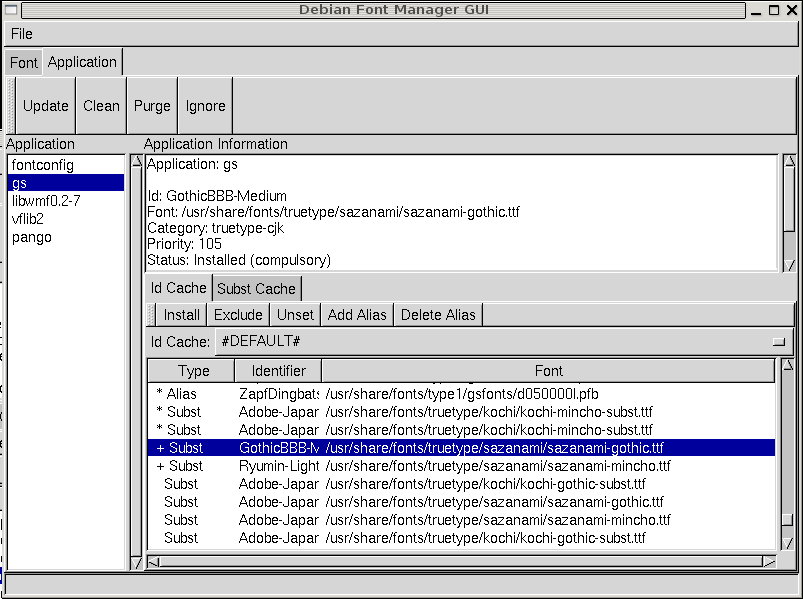
\includegraphics[width=12cm]{image200604/dfontmgr.png}

\end{itemize}

それぞれの方法にハイパーリンクやpstricksの扱いに癖があります。
たとえば、dvipdfmxの場合はhyperrefパッケージを読み込む際に、dvipdfmオプ
ションを指定してあげる必要があります。

\begin{commandline}
 \usepackage[dvipdfmx]{hyperref}
\end{commandline}

\subsection{jlatex}

jlatexは、jtex-binパッケージに入っています。
texファイルからdviファイルを生成することができます。

ただ、platex向けの既存のドキュメントをコンパイルしようとしてもエラーにな
ります。 Debian勉強会資料で利用している jsarticle.cls や ascmac.sty など
がplatex専用だからのようです。 j-articleなどを利用する必要があるようです
\footnote{jarticle は利用できるようになっている。}。また、このドキュメン
トに関してはそれ以外にも問題があり、簡単な変更では処理できませんでした。

\begin{commandline}
 $ jlatex debianmeetingresume200604.tex
! LaTeX Error: File `jsarticle.cls' not found.
(エラーがでてコンパイルできない)
\end{commandline}

\subsection{cjk-latex}

babelのCJKパッケージとして実装されており、通常のlatexを利用して日本語を
処理できるそうです。

そのままでは \texttt{/usr/share/doc/cjk-latex/examples} にあるサンプルファ
イルすらコンパイルできないので、困りものです。

参考:
\url{http://lists.debian.or.jp/debian-devel/200007/msg00150.html}

\subsection{pdfelatex}

Debianには部品が現状足りないようです。

参考:
\url{http://cise.edu.mie-u.ac.jp/~okumura/texfaq/qa/17780.html}

\subsection{multex}

パッケージをインストールしただけでは、サンプルファイルを処理してもフォン
トが一部足りないようで、表示されない文字があります。

参考:
\url{http://lists.debian.or.jp/debian-users/200106/msg00081.htm}

\subsection{lambda (omega)}

\url{http://www.fsci.fuk.kindai.ac.jp/kakuto/soft.html}、
\url{http://cise.edu.mie-u.ac.jp/~okumura/texfaq/japanese/}などを参考に
してみてください。現状、実用的に既存のドキュメントをそのまま処理できるよ
うな形式ではないことがうかがえます。

\dancersection{次回}{}

5月14日にオンラインで開催予定です。
Debian Conferenceの状況と抱負をお伝えできる予定です。

参加者募集はまた後程。

\newpage

\vspace*{15cm}
\hrule
\vspace{2mm}

\includegraphics[width=2cm]{image200502/openlogo-nd.eps}
\noindent \Large \bf Debian 勉強会資料\\ \\
\noindent \normalfont 2006年4月15日 \hspace{5mm}  初版第1刷発行\\
\noindent \normalfont 東京エリア Debian 勉強会 (編集・印刷・発行)\\
\hrule

\end{document}
